\chapter{Network Layer - Piano dei dati}

\section{I router}
I router sono sicuramente i dispositivi più responsabili dell'instradamento e dell'inoltro all'interno delle reti. Sono quindi un elemento fondamentale per il Network Layer, e quindi da studiare approfonditamente.

\subsection{Elementi principali di un router}
\begin{figure}[htp]
	\centering
	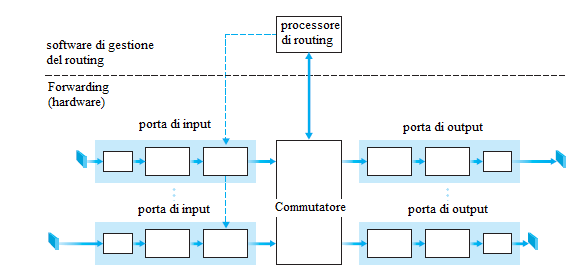
\includegraphics[width=0.75\linewidth]{./images/router.png}
\end{figure}

\begin{itemize}
	\item \textbf{Porte di ingresso.}\\
	Sono le \textbf{terminazioni a livello fisico} per i collegamenti in ingresso al router. Inoltre, è sempre nella porta d'ingresso che si effettua la \textbf{decisione di forwarding}. Ogni porta contiene infatti una copia della tabella di routing.
	In questo caso, il termine "porta" fa riferimento a interfacce fisiche d'input (e output), ben diversi dalle porte software dei processi e dei socket.
	
	\item \textbf{Struttura di commutazione.}\\
	Connette fisicamente le porte d'ingresso a quelle di uscita. Una sorta di rete interna al router. È una struttura che deve permettere una \textbf{commutazione ad alta velocità}, sfruttando la tabella di forwarding fornita dal piano di controllo.
	
	\item \textbf{Porte di uscita.}\\
	Memorizzano i pacchetti che provengono dalla struttura di commutazione e li trasmettono sul collegamento d'uscita. Nei collegamenti bidirezionali, la porta d'uscita è accoppiata alla porta d'ingresso sulla stessa scheda di collegamento (detta line card).
	
	\item \textbf{Processore d'instradamento.}\\
	Esegue le funzioni del piano di controllo. Il funzionamento varia tra i router tradizionali e quelli SDN\footnote{Software Defined Networking}. Nei primi, il processore d'instradamento gestisce le tabelle di inoltro. Nel secondo caso, si occupano di gestire la comunicazione con il controller remoto.
\end{itemize}

In un router, mentre il processore d'instradamento è principalmente software, le porte di ingresso, di uscita e le strutture di commutazione, sono gestite da hardware dedicato.
In questo modo, è possibile ottenere le performance richieste dalla rete, operando in lassi temporali dell'ordine dei millisecondi. 

\newpage
\subsection{Porte d'ingresso del router}
Le porte d'input svolgono sia una funzione di terminazione (elettrica) per il livello fisico, sia l'elaborazione per il livello di collegamento.\\
Usando le informazioni della tabella d'inoltro, viene determinata la porta d'uscita dei pacchetti (attraverso la struttura di commutazione).\\
La tabella di inoltro viene elaborata e aggiornata dal processore di instradamento (control plane), e viene copiata e mandata a line card e porte d'ingresso, in modo da permettere alle porte d'ingresso di prendere decisioni senza invocare il processore d'instradamento centralizzato.

\subsection{Tabelle d'inoltro e destination-based forwarding}
\begin{figure}[htp]
	\centering
	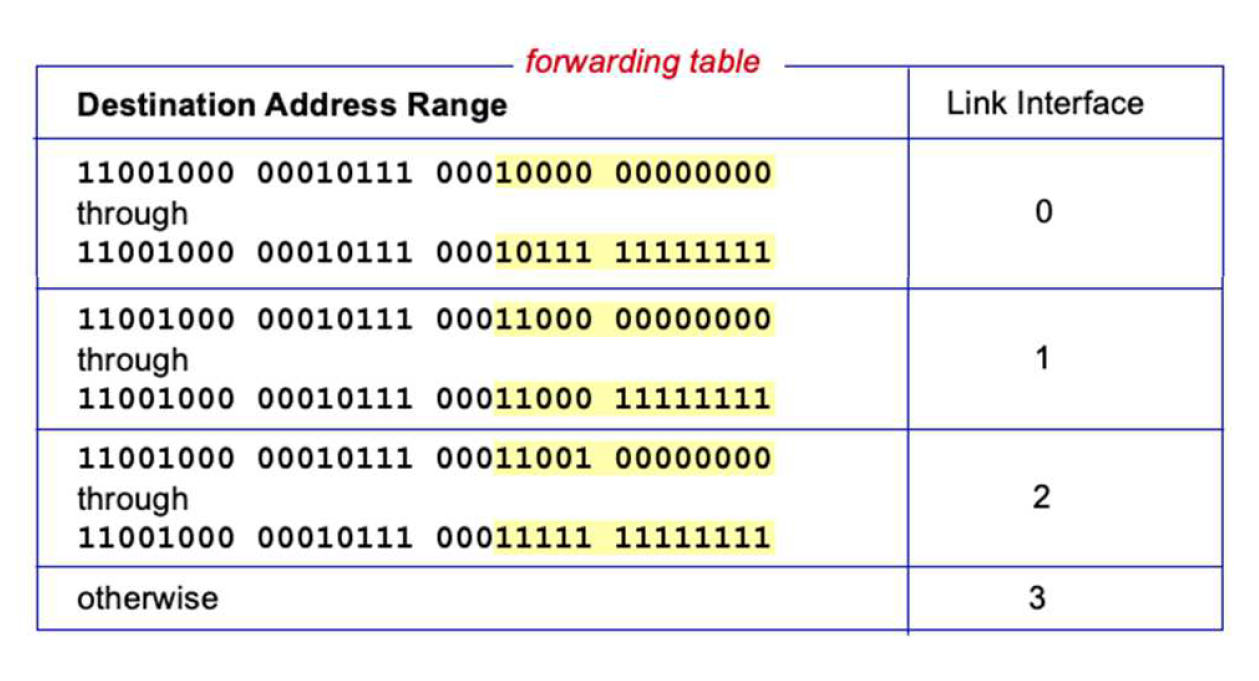
\includegraphics[width=0.75\linewidth]{./images/tabellainoltro.png}
\end{figure}
La decisione della porta d'inoltro può avviene tramite un processo di longest-prefix-matching (in italiano, corrispondenza a prefisso più lungo). L'indirizzo di destinazione viene confrontato con una lista di prefissi associati a dei collegamenti: quello dal match migliore, detterà la porta d'uscita dei pacchetti.
\begin{figure}[htp]
	\centering
	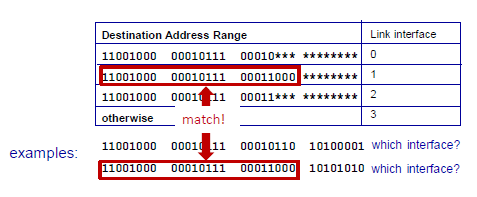
\includegraphics[width=0.75\linewidth]{./images/prefix.png}
\end{figure}

\subsubsection{Ternary Content Addressing Memory}
Lo string matching non è un problema semplice, nemmeno nel caso dei prefissi: soprattutto in un contesto come quello dei router, che devono operare ad altissime velocità, risulta fondamentale implementare questi meccanismi in maniera hardware.\\
Entrà quindi in giorno la TCAM. La Ternary Content-Addressable Memory (TCAM) è un tipo specializzato di memoria ad alta velocità che può cercare all'interno del suo intero contenuto in un solo ciclo di clock. Il termine ternario si riferisce alla capacità della memoria di memorizzare e interrogare i dati utilizzando tre diversi valori: 0, 1 e X (perfetta per i prefissi!). La TCAM è utilizzata nel contesto dei router per memorizzare le tabelle di ricerca degli indirizzi, ed effettuare in tempo costante il controllo di tutti i prefissi, per trovare il prefisso dal matching migliore con l'indirizzo di destinazione fornito.

\newpage

\subsection{Struttura di commutazione}
È il cuore del router, mezzo tramite cui i pacchetti vengono commutati (inoltrati) dalla porta d'ingresso alla porta d'uscita. La commutazione può essere ottenuta attraverso varie strutture di commutazione:
\begin{itemize}
	\item \textbf{Commutazione in memoria.}\\
	Avviene sotto il controllo diretto della CPU (ovvero il processore di instradamento), con le porte di ingresso e uscita trattate come dispositivi di I/O. I primi router usavano questa struttura, che con una determinata bandwidth della memoria tale da permettere di leggere e scrivere $B$ pacchetti per unità di tempo, il throughput complessivo d'inoltro deve necessariamente essere $< \frac{B}{2}$. Le operazioni di inoltro su due porte differenti non potevano nemmeno avvenire in contemporanea, a causa dell'impossibilità di effettuare due operazioni di lettura/scrittura contemporaneamente.\\
	Alcuni router attuali effettuano commutazione in memoria, ma la ricerca dell'indice e la memorizzazione del pacchetto nella locazione di memoria opportuna avviene sulle line card di ingresso. Alcuni di questi router, somigliano a sistemi multiprocessore a memoria condivisa.
	
	\item \textbf{Commutazione tramite bus.}\\
	In questo approccio le porte di ingresso trasferiscono un pacchetto direttamente alle porte di uscita tramite un bus condiviso e senza intervento dal processo di instradamento.\\
	Si ottiene aggiungendo al pacchetto un'etichetta di commutazione: questa indicherà la porta locale di output da cui dovrà uscire. Il pacchetto verrà ricevuto da tutte le porte d'output, ma solo la porta corrispondente lo raccoglierà. Un difetto di questo sistema? Solo un pacchetto alla volta può occupare il bus: la larghezza di banda della commutazione sarà limitata da quella del bus. Più pacchetti da commutare saranno messi in coda. È comunque un valido sistema per router in reti di accesso e aziendali. Gli switch Cisco della serie 5600 hanno una bandwidth di $32 \ Gbps$.
	
	\item \textbf{Commutazione attraverso rete di interconnessione.}\\
	Usa una rete di interconnessione più sofisticata, con una matrice di commutazione (\textit{crossbar switch}): consiste in $2n$ bus che collegano $n$ porte di ingresso a $n$ porte d'uscita. Ogni bus verticale interseca tutti i bus orizzontali a un punto d'incrocio che può essere aperto o chiuso dal controller della struttura di commutazione in qualsiasi momento.
	Quando un pacchetto che entra dalla porta $A$ deve essere inoltrato alla porta d'uscita $Y$, viene chiuso l'incrocio tra i bus $A-Y$.\\ Analogamente, questo avviene per l'entrata $B$ e l'uscita $X$. Quando sono coinvolte porte d'uscita differenti, i pacchetti possono essere trasferiti in parallelo, altrimenti si accoderanno alla porta d'output.\\
	Architetture più sofisticate utilizzano strutture per la commutazione a più stadi, che permette di spostare in contemporanea pacchetti da più porte verso una sola porta.\\
	Tra questi, i router Cisco CRS usano un'ulteriore strategia a $n$ strutture di commutazione: il pacchetto da trasferire viene suddisivo in $k$ frammenti (chunk). Ogni frammento verrà trasferito attraverso una struttura, mentre la porta di uscita si occuperà del riassemblaggio. Questo permette di avere ancora $n-k$ strutture di commutazione libere per eventuali altri pacchetti.
	\begin{figure}[htp]
		\centering
		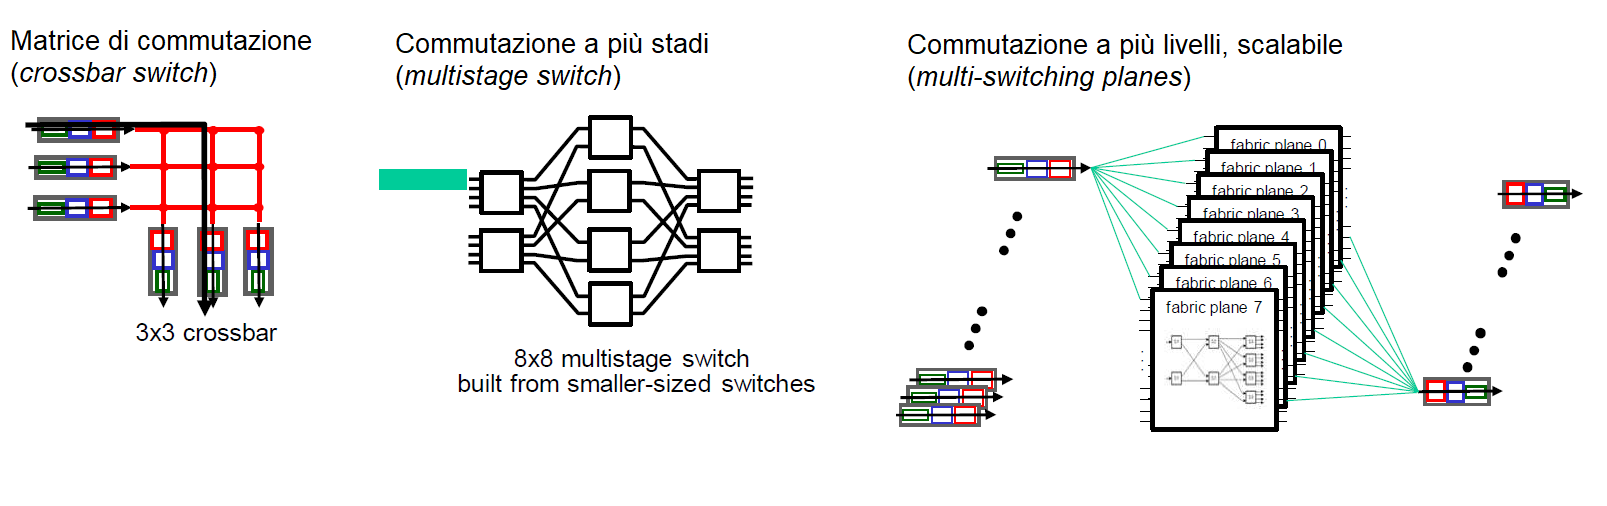
\includegraphics[width=1\linewidth]{./images/commutationstructure.png}
	\end{figure}
\end{itemize}

\newpage

\subsection{Accodamento}
L'accodamento è un fenomeno che, se non viene gestito correttamente, può portare alla saturazione totale della memoria e alla perdita di pacchetti.

\subsubsection{Accodamento alle porte d'ingresso}
Quando la struttura di commutazione non è sufficientemente rapida rispetto alle linee di ingresso, è proprio nelle porte d'input che si ha accodamento. I pacchetti sono serviti con un meccanismo FCFS (\textit{First-Come-First-Served}).\\
Abbiamo già detto che pacchetti che devono uscire da porte differenti possono essere trasferiti in parallelo. Quando due pacchetti devono uscire dalla stessa porta, uno dei due dovrà attendere. Supponiamo di avere due porte $A, B$ e due uscite $X,Y$. Supponiamo arrivino due pacchetti $x_1, x_2$ per $X$, uno dalla porta $A$, uno dalla porta $B$. Se $x_1$ va verso la porta $X$, $x_2$ andrà in coda. Un eventuale pacchetto $y_1$ che dalla porta $B$ vuole andare alla porta $Y$ soffrirà di un fenomeno noto come \textbf{HOL blocking}, proprio a causa dell'accodamento di $x_2$.

\subsubsection{Accodamento alle porte d'uscita}
Supponiamo che $R_{switch}= N \cdot R_{line}$, ovvero che il tasso di trasferimento della struttura sia $N$ volte più veloce della velocità di trasferimento nelle linee d'input e output.\\
Nel tempo richiesto per ricevere o trasmettere un pacchetto, una porta potrebbe ricevere fino a $N$ pacchetti, causando la formazione di una coda nella porta d'uscita. Il numero di pacchetti nella coda d'uscita è direttamente proporzionale alla dimensione del buffer di quella porta. Quando il buffer è saturo e arriva un ulteriore pacchetto, si deve stabilire se effettuare un \textbf{drop-tail}, scartando il nuovo pacchetto, o rimuoverne uno o più di uno tra quelli già in coda, a favore del nuovo arrivato.

\subsubsection{Quanta memoria assegnare al buffer}
\verb|RFC 3439| stabiliva che la grandezza del buffer $B$ dovesse essere uguale al round trip time medio $RTT$ moltiplicato per la calacità del link $C$.\\
Un esempio? Un collegamento con bandwidth $10 \ Gbps$ con un RTT di $250 \ ms$ necessiterebbe di un buffer $B$ pari a
$$
B = RTT \cdot C = 10 \ Gbps \cdot 250 \ ms = 10 \cdot 0,25 = 2,5 \ Gbit
$$
Anche se recenti studi teorici, suggeriscono che, con un numero $N$ di flussi TCP indipendenti, la quantità di buffer necessaria sia 
$$
B \approx RTT \cdot \frac{C}{\sqrt{N}}
$$
Buffer troppo grandi aumentano i delay (soprattutto nei router di casa, che non gestiscono in maniera ottimale la coda, causando \textbf{bufferbloat}).
RTT troppo lunghi rendonono i mittenti TCP meno reattivi. Alcuni controlli della congestione basati sul ritardo permettono di mantenere la linea occupata, senza riempire il buffer.

\begin{figure}[htp]
	\centering
	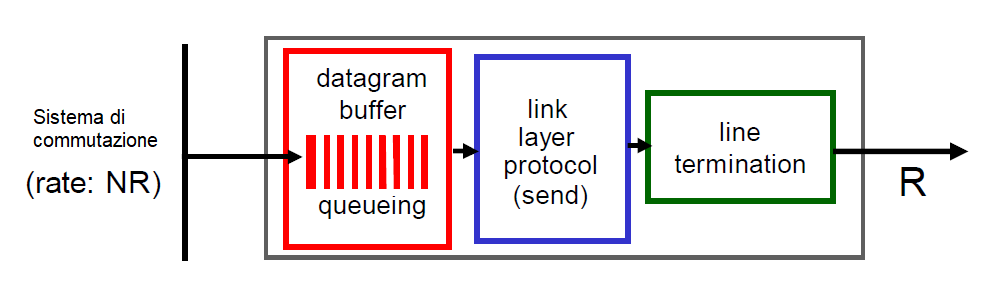
\includegraphics[width=0.75\linewidth]{./images/portaduscita.png}
\end{figure}


\newpage

\subsection{Packet discarding policy}

\subsubsection{Tail drop}
Quando la coda è piena, \textbf{i pacchetti in arrivo vengono scartati a priori}, senza considerare priorità o tipologia del traffico. Droppare pacchetti in questo modo potrebbe causare \textbf{burst di drop}.

\subsubsection{Priority queueing}
Il buffer è diviso in più code, ognuna con priorità diversa. I pacchetti vengono etichettati con un livello di priorità (o può essere stabilita dal router). In questo modo, i pacchetti ad alta priorità non saranno scartati, quando sono presenti in coda altri pacchetti a priorità più bassa. 

\subsection{Scheduling dei pacchetti}
Come determiniamo l'ordine con cui trasmettere i pacchetti su una determinata porta d'uscita? 

\subsubsection{FIFO (o FCFS)}
First-In-First-Out o First-Come-First-Served. Il paradigma più semplice: chi prima arriva, prima viene mandato.

\subsubsection{Priority scheduling}
Estende il modello FIFO-FCFS con un meccanismo di priorità: vengono definite più code per varie classi di priorità. Ad esempio, con due code (alta e bassa priorità), è possibile distribuire i pacchetti dei servizi in tempo reale (o informazioni di gestione di rete) e i pacchetti di servizi non in tempo reale. Le singole code seguono solitamente il principio FIFO, ma, date due code non vuote, verrà sempre preso il pacchetto nella coda ad alta priorità.

\subsubsection{Round-Robin}
Vengono di nuovo suddivisi i pacchetti in classi, non più (mandatoriamente) suddivise per priorità di servizio. A turno, ogni coda viene servita: viene trasmesso un pacchetto di classe $1$, poi $2$, fino alla $n$-esima classe. Poi di nuovo $1$, $2\dots n$. Col \textit{work-conserving round robin}, quando una coda è vuota, viene del tutto saltata dalla selezione.
%Adoro i bambini 

\subsubsection{WFQ - Weighted Fair Queuing}
Accodamento equo ponderato. È un Round Robin generalizzato, in cui ogni classe può ricevere un servizio differenziato. Ogni classe $i$ avrà un peso $w_i$. Il WFQ assicura che l'$i$-esima classe di pacchetto riceva sempre $\frac{w_i}{\sum{w_i}}$, dove $\sum w_i$ indica la somma tra i pesi di tutti i servizi.\\
Non dimentichiamo, tuttavia, che i pacchetti sono unità discrete e che la loro trasmissione non può essere interrotta. Questo rapporto è quindi indicativo.

\section{I protocolli del livello di rete}
\begin{itemize}
	\item \textbf{IP protocol}.\\
	E la formattazione dei pacchetti, l'addressing e le convenzioni relative alla gestione dei pacchetti.
	\item \textbf{Path-selection algorithm.}\\
	Che gestiscono l'instradamento dei pacchetti.
	\item \textbf{Protocollo ICMP}.\\
	Dedicato agli errori e ai segnali dei router.
\end{itemize}

\newpage

\section{IPv4 - Internet Protocol v4}

\subsection{Indirizzo IP}
Un indirizzo IP è un codice logico (non fisico, non 1-a-1) associato ad un host connesso a una rete che usa il protocollo Internet. 

\subsubsection{Classi di indirizzi IP}
Un sistema che permetteva di distinguere vari tipi di indirizzi IP è quello per classi.
\begin{itemize}
	\item Indirizzi di classe A.\\
	From \verb|1.0.0.0| to \verb|127.255.255.255|.
	Il primo byte identifica la rete, gli altri gli host.
	\item Indirizzi di classe B.\\
	From \verb|128.0.0.0| to \verb|191.255.255.255|.
	I primi due byte identificano la rete, gli ultimi due gli host.
	\item Indirizzi di classe C.\\
	From \verb|192.0.0.0| to \verb|223.255.255.255|
	I primi tre byte identificano la rete, l'ultimo gli host.
	\item Indirizzi di classe D (multicast).\\
	From \verb|224.0.0.0| to \verb|239.255.255.255|. Sono riservati agli indirizzi multicast. Permettono quindi di trasmettere la stessa informazione a più dispositivi contemporaneamente senza dover duplicare l'informazione.
	\item Indirizzi di classe E (riservati).\\
	Riservati per usi futuri.
	From \verb|240.0.0.0|
\end{itemize}

\subsubsection{Alcuni indirizzi specifici}
Questi indirizzi sono riservati a delle funzioni specifiche.
\begin{itemize}
	\item \verb|0.0.0.0| - This Host, usato su un host cui indirizzo non è ancora stato specificato (ma solo in IPv4, non in IPv6, che usa un indirizzo IP basato sul MAC Address. Guarda EUI-64, pagina 81).
	\item \verb|255.255.255.255| - Broadcast relativo alla propria subnet.
	\item \verb|127.0.0.0 - 127.255.255.255| - Localhost, riferimento a se stesso.
	\item \verb|10.0.0.0 - 10.255.255.255| - Private IP.
	\item \verb|169.254.0.0 - 169.254.255.255| - Automatic Private IP Addressing (APIPA), usate per risolvere problemi relativi al DHCP.
\end{itemize}

\subsection{Assegnamento degli indirizzi IP}
\begin{enumerate}
	\item Inizialmente, questo compito era affidato alla \textbf{IANA} (Internet Assigned Numbers Authority), ai tempi di Arpanet.
	\item Nel 1992, sono stati creati i \textbf{RIR} (Regional Internet Registers), creati per gestire gli indirizzi e domini per ogni area assegnata
	\item Nel 1998 un'associazione non-profit chiamata \textbf{ICANN} (Internet Corporation for Assigned Network and Numbers) è stata fondata per coordinare tutti i RIR del mondo.
\end{enumerate}

\subsubsection{I RIR attuali}
\begin{itemize}
	\item APNIC - Asia Pacific Network Information Center
	\item ARIN - American Registry for Internet Numbers
	\item LACNIC - Latin American and Caribbean Internet Addresses Registry
	\item RIPE NCC - Réseaux IP Européens Network Coordination Centre
	\item AFRINIC - African Regional Internet Registry
\end{itemize}

I RIR sono responsabili per i Local Internet Registries, che gestiscono gli indirizzi a livello locale. Un esempio è il GARR-LIR\footnote{GARR è il nome della rete italiana a banda ultralarga dedicata alla comunità dell'istruzione, della ricerca e della cultura (NREN), oltre che del consorzio che la gestisce.}. I RIR forniscono vari set di indirizzi (statici e dinamici) agli ISP.


\newpage

\subsection{Formattazione dei Datagram IPv4}
Questa è la struttura di un datagramma IPv4. Osserviamo i singoli campi

\begin{figure}[htp]
	\centering
	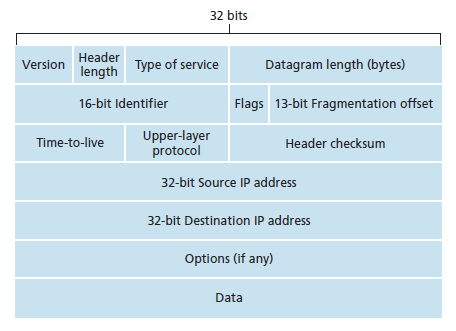
\includegraphics[width=0.75\linewidth]{./images/ipv4datagram.png}
\end{figure}


\begin{itemize}
	\item \textbf{Version.}\\
	Indica la versione di IP usata dal datagramma. È fondamentale per capire come interpretare il pacchetto IP. 4 bit. 
	\item \textbf{Internet Header Length.}\\
	Indica la lunghezza dell'header del pacchetto IP, ovvero l'offset del campo dati, che varia da 5 word a 15 word (ovvero da 20 a 60 byte). Ciò dipende dalla presenza o meno del campo \textit{Options}.
	\item \textbf{Type of Service.}\\
	Da informazioni relative al servizio fornito, stabilendone la priorità.
	
	\item \textbf{Datagram length.}\\
	Indica la dimensione in byte dell'intero pacchetto. Include quindi header e dati. 16 bit.
	
	\item \textbf{ID, Flags e Fragmentation Offset.}\\
	Ne parleremo meglio dopo. Rispettivamente 16, 3 e 13 bit.
	
	\item \textbf{TTL - Time To Live.}\\
	Specifica il tempo di vita massimo di un pacchetto. Per qualsiasi problema nella rete, un pacchetto potrebbe persistere nella vita per un quantitativo spropositato di tempo. Potrebbe essere addirittura una cosa voluta per un possibile attacco hacker. Il time to live ovvia a questo problema definendo un numero di salti, nel momento in cui il pacchetto viene mandato in rete: ogni salto attraverso un router implica un decremento. Usa 8 bit.
	
	\item \textbf{Protocol.}\\
	Specifica il protocollo del transport layer. 4 bit.
	
	\item \textbf{Header checksum.}\\
	8 bit dedicati alla somma di controllo. Un pacchetto cui header risulta corrotto, viene scartato. Le operazioni sono di natura logica o matematica, ed il controllo è fatto a ogni router.
	
	\item \textbf{Options.}\\
	Quasi inutilizzate.
	
	\item \textbf{Source IP e Destination IP.}\\
	32 bit ciascuno, 64 in totale. Sono due campi separati.
\end{itemize}

\subsection{Un problema: la frammentazione}
Alcuni campi che non abbiamo ancora affrontato, sono quelli relativi alla frammentazione. Quando un datagramma IP viene frammentato in più datagrammi IP più piccoli, queste informazioni permettono la ricostruzione del frammento originale a destinazione.
La frammentazione avviene quando un router ha MTU (Max Transfer Size) tale da non consentire il trasferiremnto dell'intero datagramma IP.
\begin{itemize}
	\item \textbf{ID.}\\
	16 bit, identificano un insieme di pacchetti IP che (presumibilmente) ricostruiranno un pacchetto originale.
	\item \textbf{Flags.}\\
	3 bit, 2 usati. I flags sono \verb|DF - Don't Fragment|, $=1$ "Non frammentare mai. Al massimo, scarta."\\
	\verb|MF - More Fragments|, $=1$ "Questo non è l'ultimo frammento".
	\item \textbf{Offset.}\\
	13 bit, indica dove inizia il frammento rispetto all'inizio del pacchetto originale, espresso in unità da 8 bit. Permette di ricostruire in maniera opportuna i pacchetti frammentati.
\end{itemize}

Questo compito non spetta solitamente ai router, i quali ricordiamo occuparsi principalmente di forwarding. Una corruzione dei dati di frammentazione può avere gravi conseguenze in fase di ricostruzione.

\begin{itemize}
	\item \textbf{Offset alterato} - il ricongiungimento dei pezzi non può essere eseguito correttamente.
	\item \textbf{ID alterato} - un frammento potrebbe cambiare pacchetto di appartenenza.
	\item \verb|MF=1 -> MF=0| - un frammento che non è l'ultimo potrebbe essere considerato l'ultimo.
\end{itemize}

\subsubsection{Esempio di frammentazione}
Dato un pacchetto con 4000 byte e un router con MTU di 1500 byte (come Ethernet).
\begin{itemize}
	\item Se il frammento arriva con il flag $\verb|DF|= 1$, viene scartato
	\item Con $\verb|DF|=0$ si procede alla frammentazione.
\end{itemize}

Vediamo come procederebbe la frammentazione.

\begin{enumerate}
	\item Il primo frammento viene mandato con $\verb|MF|=1$ con offset a 0. Il segmento mandato è di 1480 byte, in quanto 20 byte saranno occupati dall'header TCP. $4000-1480 = 2520$ byte da mandare rimanenti.
	
	\item Il secondo frammento viene mandato con $\verb|MF|=1$ con offset a $\frac{1480}{4}=370$.  $2520-1480 = 1040$ byte da mandare rimanenti.
	
	\item Il terzo frammento viene mandato con $\verb|MF|=0$ ($1040-1480 < 0$) con offset a $\frac{1480}{2}=740$.  
\end{enumerate}




\newpage

\subsection{Indirizzamento IPv4}
Abbiamo detto che un indirizzo IP identifica univocamente un dispositivo. Ciò è improprio: gli indirizzi IP identificano un'interfaccia di rete. Se i  computer hanno una sola interfaccia di rete, e quindi un solo indirizzo IP, i router presentano $n$ interfacce, e quindi $n$ indirizzi IP. Ogni indirizzo IP identifica una subnet.
Gli indirizzi IPv4 hanno lunghezza di 32 bit. Avremo quindi $2^{32}$ indirizzi.

Gli indirizzi IP usano la seguente notazione : \verb|193.32.216.9|, detta notazione decimale puntata. Ogni interfaccia di host e router di Internet ha un indirizzo IP globalmente univoco (fatta a eccezione di quelle gestite da NAT, di cui parleremo più avanti).

\subsubsection{Come vengono determinati gli indirizzi IP}
Gli indirizzi IP non sono determinati in maniera arbitraria. Parte dell'indirizzo IP di una determinata interfaccia dipende dalla sottorete a cui è collegata. Questa struttura non arbitraria è la chiave dietro al funzionamento degli indirizzi IP.

\begin{figure}[htp]
	\centering
	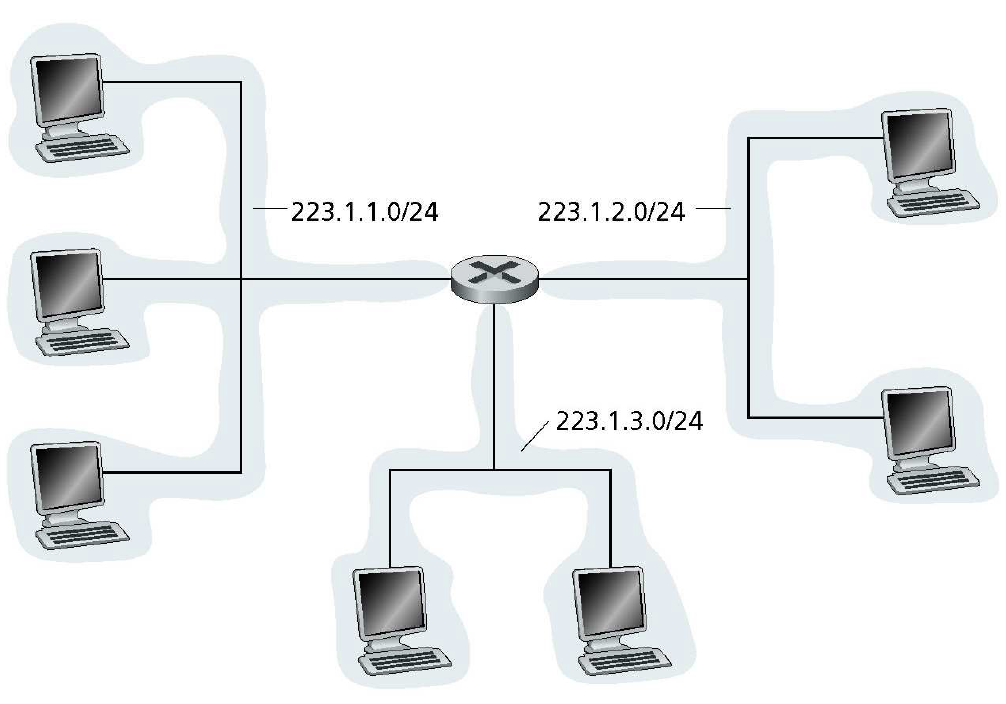
\includegraphics[width=0.5\linewidth]{./images/reteip.png}
\end{figure}

L'interfaccia di rete di un router e i dispositivi a essa collegata (magari tramite uno switch o da un punto di accesso Wireless) costituiscono una sottorete [RFC 950]. Ad esempio, IP assegna ad una sottorete l'indirizzo \verb|223.1.1.0/24|. La notazione \verb|/24| è chiamata maschera di rete, ed indica che i 24 bit più a sinistra dell'indirizzo definiscono l'indirizzo della sottorete. Questo vuol dire che tutti i dispositivi partecipanti a questa rete avranno indirizzo IP nella forma \verb|223.1.1.XXX|\footnote{Con XXX nel range $[2-254]$, escludendo $0$ in quanto \textit{forbidden}, 1 riservato ai router e 255 per il broadcast}.



\subsubsection{Regola generale per individuare sottoreti}
\textit{Per determinare le sottoreti, si sgancino le interfacce da host a router in maniera tale da creare isole di reti isolate delimitate dalle interfacce. Ognuna di queste reti isolate viene detta sottorete.}

\newpage
\subsection{CIDR - Classless InterDomain Routing}
CIDR [RFC 4623] (pronunciato \textit{Cider}) generalizza l'indirizzamento di sottorete nel seguente modo:

\begin{itemize}
	\item L'indirizzo IP è nella forma $a.b.c.d/x$
	\item $x$ indica il numero di bit della prima parte dell'indirizzo.
	\item La prima porzione è detta porzione di rete, o prefisso, dell'indirizzo IP. 
	\item La seconda porzione (di $32-x$ bit) distingue i dispositivi all'interno della stessa rete, o delle ulteriori sottoreti.\\
	\textit{Un esempio? La rete denotata da $a.b.c.d/21$ contiene anche la sottorete denotata da $a.b.c.d/24$, all'interno della stessa organizzazione.}
\end{itemize}

Questo metodo è stato introdotto dopo l'utilizzo del classful addressing, che segue la suddivisione in classi che abbiamo introdotto precedentemente.\\ Detto ciò, la suddivisione meno rigida del CIDR ha permesso alle aziende di scegliere un valore di $x$ che minimizzi lo spreco di indirizzi IP, ottenendone invece un quantitativo che rispecchi quanto possibile le esigenze del sistema.

\subsubsection{Da una domanda su stack overflow}

\begin{small}
	\begin{verbatim}
		Class based addressing basically divides the total IPv4 range into five classes: 
		Class A through E; Whereas CIDR is based on concept of subnetting.
		
		Your company wants 32 public ip addresses.
		If we assign them a class C address, for example 192.168.2.0, their company 
		reserves all IP addresses in range 192.168.2.1 - 192.168.2.254. 
		
		But they only want 32 ip addresses which means 223 addresses will be wasted.
		This is the constraint of classful addressing. Now if we look at just subnetting, 
		class c ip address has default subnet of 255.255.255.0 so if we divide the range of 
		192.168.2.0 in 6 subnets each containing 32 available ip addresses your problem 
		is solved. 
		
		But, if we take this example to higher level we will require CIDR.
		According to traditional subnetting, we can not combine the addresses from the networks 
		192.168.2.0 and 192.168.3.0 because the netmask for class C addresses is 255.255.255.0. 
		However, using CIDR notation, we can combine these blocks by referencing this chunk as 
		192.168.2.0/23.
		
		This specifies that there are 23 bits used for the network portion that we are 
		referring to. 
		With this, the 24th bit can be either 0 or 1 and it will still match, because the 
		network block only cares about the first 23 digits.
		
		CIDR allows more control over addressing continuous blocks of IP addresses. 
		This is much more useful than the subnetting we talked about originally.
	\end{verbatim}
\end{small}
\subsubsection{IP broadcast}
\verb|255.255.255.255|. Quando un host emette un datagramma con tale IP destinazione, il messaggio viene consegnato a tutti gli host sulla stessa sottorete.



\newpage

\subsection{Come vengono usate le maschere di rete}
La maschera di rete, indicata in notazione CIDR con $/x$ indica che i primi $x$ bit a sinistra indicano la (sotto)rete. Nella maschera di rete, i primi $x$ bit a sinistra saranno 1, gli altri $32-x$ a 0. Alcuni esempi di maschere di rete:
\begin{itemize}
	\item Con $/19$ la maschera sarà: \verb|255.255.224.0| - \verb|11111111111111111110000000000000|
	\item Con $/24$ la maschera sarà: \verb|255.255.255.0| - \verb|11111111111111111111111100000000|
	\item Con $/16$ la maschera sarà: \verb|255.255.0.0| - \verb|11111111111111110000000000000000|
\end{itemize}
\begin{figure}[htp]
	\centering
	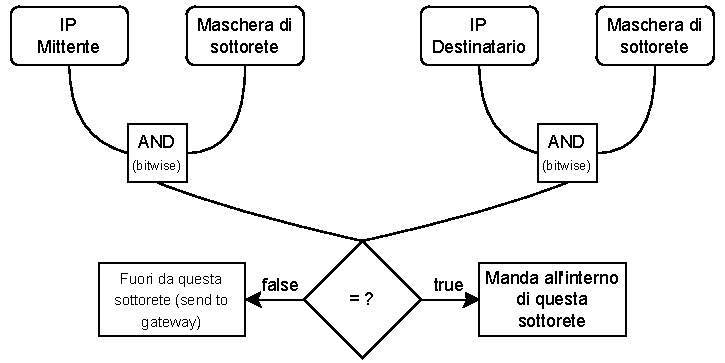
\includegraphics[width=1\linewidth]{./images/netmask.pdf}
\end{figure}
La maschera di rete può essere usata per estrapolare e confrontare l'indirizzo della sottorete di appartenenza di due host.

\newpage

\section{Elementi del livello di collegamento e ARP}
Studiando il livello di collegamento, scopriremo che gli host e i router hanno un indirizzo sia a livello di rete (IP) che a livello di collegamento (indirizzo MAC).
Il protocollo ARP (\textit{address resolution protocol}) permette  ai nodi l'associazione indirizzo IP $\to$ indirizzo MAC.

\subsection{Cos'è un indirizzo MAC?}
Un indirizzo \textit{Media Access Control} è un codice a 6 byte che identifica univocamente una scheda di rete. Gli indirizzi MAC sono univoci: la IEEE si occupa di distribuire proprio questi indirizzi MAC alle varie aziende. I primi 3 byte sono stabiliti dall'IEEE, (viene scelta quindi una combinazione di bit su $2^{24}$). Gli ultimi tre vengono dati univocamente ad ogni dispositivo prodotto dall'azienda stessa (sempre $2^{24}=16.777.216$).

\subsection{Il protocollo ARP}
Sta per \textit{Address Resolution Protocol} [RFC 826], e traduce gli indirizzi IP in MAC address. Traduce gli indirizzi IP di dispositivi situati nella stessa sottorete. Convenzionalmente, gli indirizzi IP sono scritti in decimale, gli indirizzi MAC in esadecimale.

\subsubsection{Come funziona?}
Ogni nodo contiene una tabella ARP cui record contengono tre valori: \\ \verb|Indirizzo IP - Indirizzo MAC - Time To Live|.\\
Il time-to-live specifica tra quanto tempo quel determinato record dovrà essere eliminato dalla tabella. Un tempo tipico sono 20 minuti.


\subsubsection{Caso 1 - Invio sulla stessa (sotto)rete}

\begin{enumerate}
	\item Se un datagramma deve essere mandato da un host $A$ a un host $B$ nella stessa sottorete, $A$ dovrà conoscere l'indirizzo MAC di quel dispositivo. 
	
	\item Se l'indirizzo MAC è già presente nella ARP del nodo, questo manderà il datagramma senza ulteriori passaggi.
	
	\item Altrimenti, manderà una cosidetta "richiesta ARP" contenuta in un pacchetto ARP mandato all'indirizzo broadcast della rete \verb|FF-FF-FF-FF-FF-FF|.
	
	\item Il pacchetto conterrà sia l'indirizzo IP e MAC del mittente, che l'indirizzo IP del destinatario.
	
	\item La richiesta broadcast verrà mandata a tutte le schede di rete della sottorete. La risposta ARP verrà mandata in modalità non-broadcast dal dispositivo con indirizzo IP uguale a quello della richiesta, verso il richiedente. La risposta ARP conterrà al suo interno l'indirizzo MAC del ricevente della richiesta, e la tabella ARP verrà aggiornata.
\end{enumerate}

\newpage

\subsubsection{Caso 2 - Invio su (sotto)rete diversa}
Alice desidera mandare un messaggio a Bob, collegato ad una sottorete diversa.
\begin{enumerate}
	\item Alice manda il datagramma alla sua scheda di rete. Dovrà indicare l'indirizzo MAC\\ dell'interfaccia del router a cui è collegato. Se l'indirizzo MAC è già presente nella tabella ARP di Alice, questo manderà il datagramma al router.
	
	\item Altrimenti, userà il protocollo ARP per ottenere l'indirizzo MAC. Manderà una richiesta ARP all'indirizzo broadcast della rete \verb|FF-FF-FF-FF-FF-FF|, contenente l'indirizzo IP del router.\\
	Il router, riconoscendo il proprio indirizzo, risponderà con una ARP reply condividendo ad Alice il proprio indirizzo MAC. Alice memorizzerà il nuovo indirizzo MAC appena scoperto nella propria tabella ARP, e manda il proprio frame.
	
	\begin{figure}[htp]
		\centering
		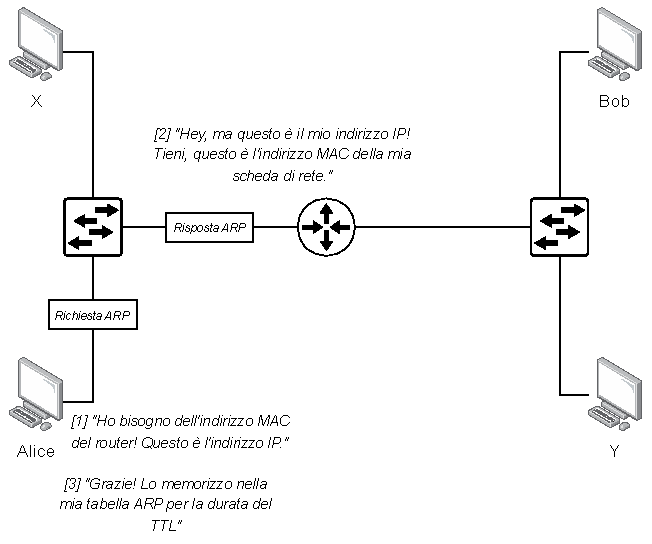
\includegraphics[width=0.75\linewidth]{./images/1-fuoridallasottorete.drawio.pdf}
	\end{figure}
	
	
	\item Il router confronta l'IP del pacchetto con la propria tabella di inoltro. Sa che il pacchetto deve essere inoltrato all'interfaccia 2, ma non conosce l'indirizzo MAC del destinatario Bob.
	
	\begin{figure}[htp]
		\centering
		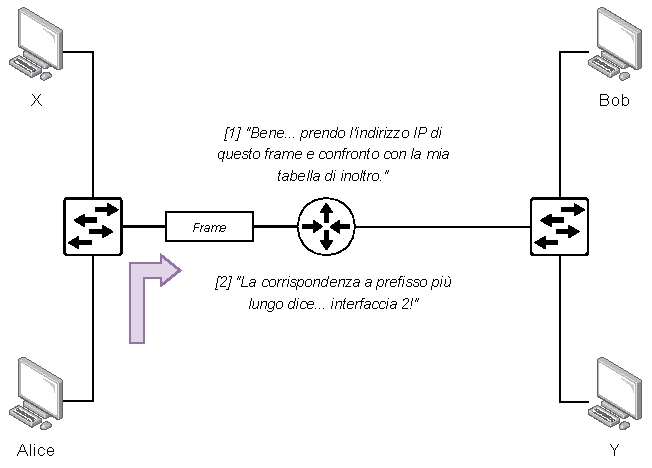
\includegraphics[width=0.75\linewidth]{./images/2-fuoridallasottorete.drawio.pdf}
	\end{figure}
	
	\newpage
	
	\item Il router manda la richiesta ARP, lo switch la manda in broadcast a tutti i dispositivi connessi. Bob riconosce l'indirizzo IP della richiesta ARP, e manda una risposta ARP. Il router riceverà l'indirizzo MAC di Bob, lo conserverà nella propria ARP table assieme al suo IP.
	\begin{figure}[htp]
		\centering
		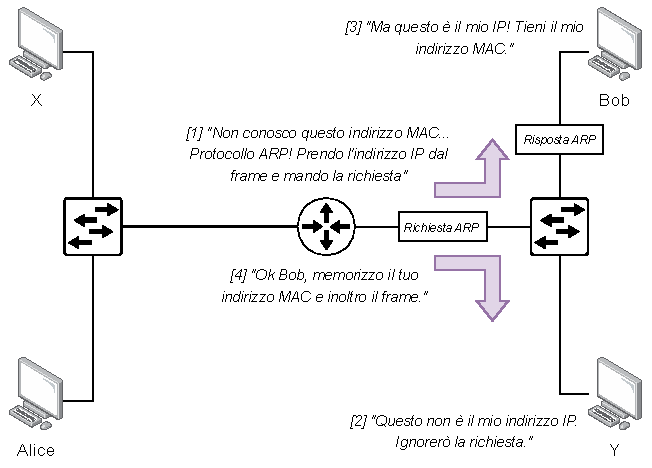
\includegraphics[width=0.75\linewidth]{./images/3-fuoridallasottorete.drawio.pdf}
	\end{figure}
	
	\item Il router avrà tutto il necessario per inoltrare il pacchetto a Bob, ed è ciò che farà.
	\begin{figure}[htp]
		\centering
		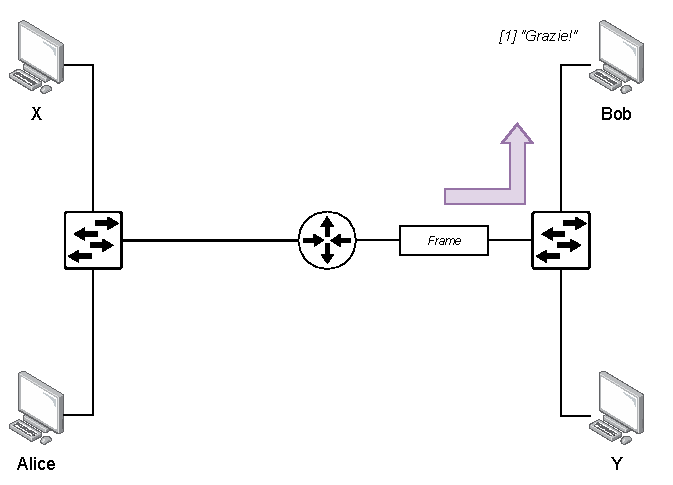
\includegraphics[width=0.75\linewidth]{./images/4-fuoridallasottorete.drawio.pdf}
	\end{figure}
	
\end{enumerate}
Notiamo che, dopo aver ottenuto tutti gli indirizzi necessari, tramite protocollo ARP, per tutta la durata delle \textit{entries} nella tabella ARP, l'inoltro sarà presumibilmente molto più veloce.

\newpage

\section{Ottenere gli indirizzi IP}
Per ottenere un blocco di indirizzi IP da usare in una sottorete, bisogna rivolgersi a Internet Service Provider (ISP). Quest'ultimo attinge da un suo blocco di indirizzi IP già allocati, e ne riserva un numero inferiore per l'ente richiedente. La dimensione della maschera di rete stabilisce la dimensione del blocco allocato.\\
L'ente che ha acquisito gli indirizzi potrà gestirseli autonomamente, costruendo le proprie sottoreti. Ogni ISP richiede uno o più blocchi di indirizzi IP all'ICANN (Internet Corporation for Assigned Names and Numbers). L'Address Support Organization si occupa dell'allocazione e della gestione degli indirizzi all'interno delle rispettive regioni, e quindi dei RIR.

\newpage
\section{DHCP - Dynamic Host Configuration Protocol}
Ottenuto un blocco di indirizzi, li si può assegnare alle interfacce dei router e degli host della propria struttura. La configurazione può avvenire manualmente, o sfruttando il \textbf{Dynamic Host Configuration Protocol} (DHCP) [RFC 2131]. Dipendentemente dalla configurazione del DHCP, gli host possono ricevere indirizzi IP persistenti e uguali a ogni accesso, o uno temporaneo.

\begin{figure}[htp]
	\centering
	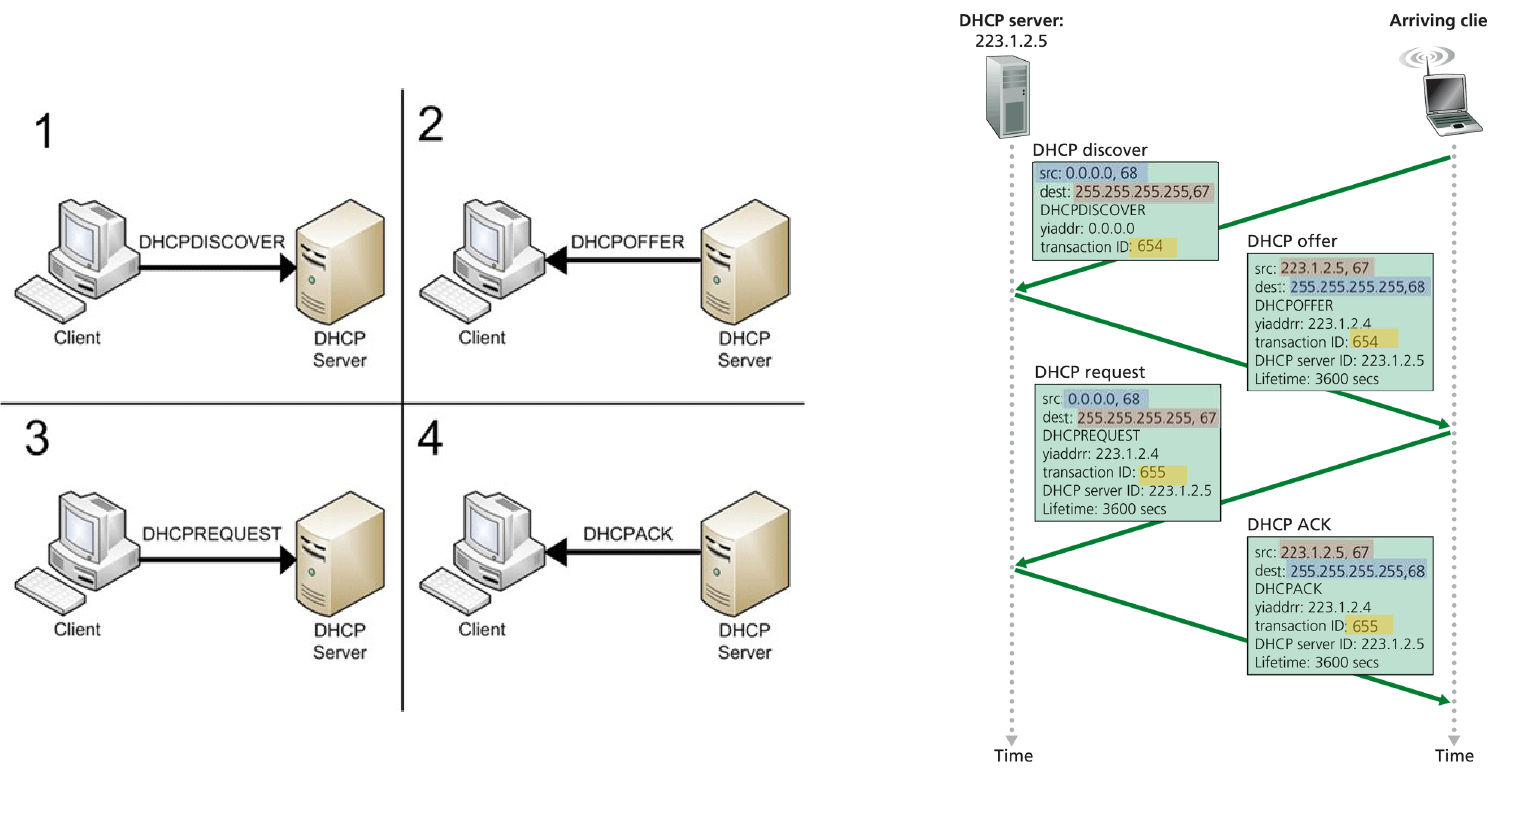
\includegraphics[width=1\linewidth]{./images/dhcp.png}
\end{figure}

\subsection{DHCP - Un protocollo plug-and-play}
Sarebbe impensabile gestire una rete (ad esempio) di un'università o di una scuola: impostare manualmente ogni dispositivo in una struttura con un alto via-vai rappresenterebbe sicuramente una criticità. DHCP imposta automaticamente un indirizzo IP per dispositivi della stessa sotto-rete.

\subsection{Come funziona DHCP}
È un protocollo client-server, in cui i client sono degli host appena connessi alla rete, richiedenti un nuovo indirizzo IP. Il server in ascolto è proprio un server DHCP, che può essere presente nella sottorete, o un relay DHCP all'interno del router che delega il lavoro ad un DHCP esterno.\\
La configurazione di un nuovo host avviene in 4 passaggi:

\begin{enumerate}
	\item \textbf{Individuazione del server DHCP.}\\
	\verb|SOURCE: IP 0.0.0.0, PORT 68  -  DESTINATION: IP 255.255.255.255 PORT: 67|.\\
	Il client manda un messaggio di tipo \textbf{DHCP discover}.
	Il messaggio è incapsulato in un \\pacchetto UDP mandato alla porta 67, e in un datagramma IP mandato in broadcasting, e quindi all'IP \verb|255.255.255.255|. Questo messaggio proviene dalla porta 68, e ha come IP del mittente l'ip \verb|0.0.0.0|.
	
	\item \textbf{Offerta del server DHCP.}\\
	\verb|SOURCE: IP dhcp_server_ip, PORT 67  -  DESTINATION: IP 255.255.255.255 PORT: 68|.\\
	Ricevuto il discover, uno o più server DHCP manderanno un broadcast \textbf{DHCP offer}.\\
	Se il client riceve più offerte, potrà scegliere quello che più preferisce. 
	L'offerta DHCP contiene l'indirizzo IP offerto, l'id transazione, l'IP del server THCP e il \textbf{lifetime} dell'IP offerto.
	
	\item \textbf{Richiesta DHCP.}\\
	\verb|SOURCE: IP 0.0.0.0, PORT 68  -  DESTINATION: IP 255.255.255.255 PORT: 67|.\\
	Il client risponde con un messaggio \textbf{DHCP request}, che riporta i parametri di configurazione.
	
	\item \textbf{Conferma DHCP.}\\
	\verb|SOURCE: IP dhcp_server_ip, PORT 67  -  DESTINATION: IP 255.255.255.255 PORT: 68|.\\
	Conferma da parte del server dei parametri richiesti con un \textbf{DHCP ACK}.
\end{enumerate}

\newpage


\newpage

\section{NAT - Network Address Translation}
\subsection{Problema da risolvere}
Ogni dispositivo ha bisogno di un indirizzo IP. Ne consegue che, al crescere del numero dei dispositivi da connettere ad una rete LAN, (apparentemente) sarà necessario avere un blocco di indirizzi di dimensione crescente. Questo approccio porta problemi: cosa si fa se necessito dall'ISP degli IP contigui che sono stati già allocati? 

\subsection{Soluzione, NAT!}
Nella rete si usa un router abilitato al NAT. A tutti i dispositivi della rete, verranno assegnati indirizzi di spazi di indirizzamento dedicati alle reti private, come lo spazio \verb|10.0.0.0/8|. Nell'esempio in questione, le nostre interfacce di rete avranno indirizzi dello spazio \verb|10.0.0.0/24|. Questi indirizzi non saranno visibili all'esterno, e quindi potranno essere riutilizzati in tutte le possibili reti private separate da router abilitati al NAT.\\
Il NAT ha il compito di tradurre gli indirizzi IP della propria sotto-rete sfruttando una NAT table, in cui i record sono del tipo
\begin{verbatim}
	
\end{verbatim}

\begin{figure}[htp]
	\centering
	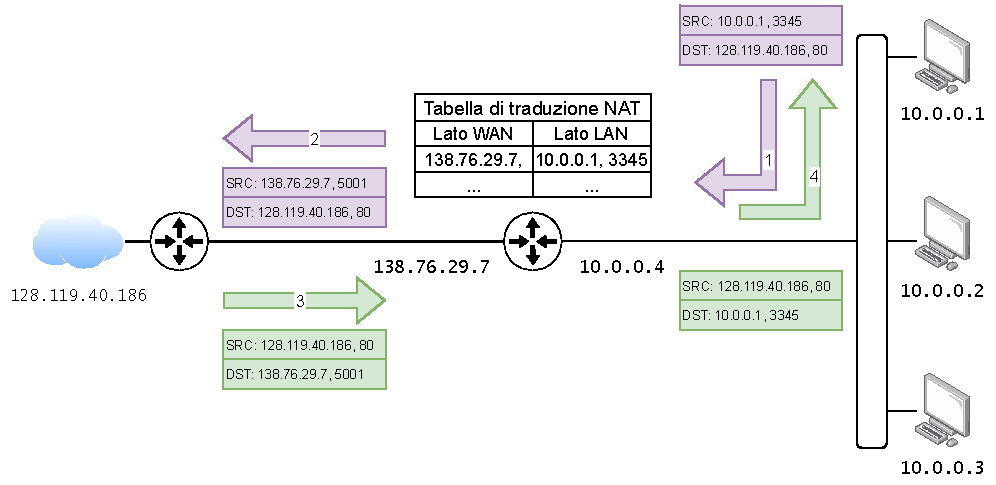
\includegraphics[width=1\linewidth]{./images/NAT.drawio.pdf}
\end{figure}

\begin{enumerate}
	\item Il router riceve i pacchetti da mandare all'esterno. Il NAT controlla se la coppia IP e porta è già presente nella tabella. Se non è presente, il NAT inserisce nella sua tabella un nuovo record, che servirà per le traduzioni. Nel lato LAN l'ip e la porta dell'interfaccia effettiva, nel lato WAN l'IP dell'interfaccia usata dal router lato WAN, e una porta generata casualmente tra quelle non usate dal quell'IP. Il NAT può gestire ben oltre 60.000 connessioni simultane con una sola interfaccia (e indirizzo IP) lato WAN!
	
	\item Il NAT controlla la propria tabella, e sostituisce IP e la porta \verb|SOURCE| del pacchetto, con quelli associati lato WAN. Inoltra regolarmente il pacchetto.
	
	\item Quando riceverà una risposta, i pacchetti arriveranno all'IP e alla porta che il NAT ha precedentemente assegnato.
	
	\item Il NAT stesso si occuperà di tradurre, dal verso opposto, la coppia IP-porta lato WAN, a quella lato LAN, inoltrando regolarmente il pacchetto.
\end{enumerate}
Il NAT non è assolutamente un protocollo perfetto. Implica una violazione del principio end-to-end, a causa della modifica dell'indirizzo IP e del numero di porta. Inoltre, causa problemi con le connessioni P2P e gli applicativi non NAT-friendly.

\newpage

\section{IPv6}
Il protocollo IPv6 nasce dall'esigenza di avere uno spazio di indirizzamento più ampio (tamponare il problema col protocollo NAT non sarebbe stato ottimale e sufficiente a lungo termine), migliorare e semplificare il protocollo IPv4. Imparando dal suo predecessore, è stato possibile creare un protocollo:
\begin{itemize}
	\item Con header più semplici.
	\item Sicuro, tramite un supporto nativo per la sicurezza (IPsec\footnote{IPsec, abbreviazione di IP Security, è uno standard per reti a pacchetto che si prefigge di ottenere connessioni sicure su reti IP. Tale sicurezza viene raggiunta attraverso l'aggiunta di funzionalità di autenticazione, cifratura e controllo di integrità dei pacchetti IP (datagrammi), incluse nell'omonima suite di protocolli e header aggiuntivi.}).
	\item Con Quality of Service migliorata.
	\item Supporto a comunicazione multicast e anycast.
\end{itemize}

\subsection{Parentesi storica}
Nei primi anni '90, si iniziò a progettare il successore di IPv4. Le motivazioni erano chiare: avere 32 bit per ogni indirizzo IP stava diventando limitante, la richiesta di indirizzi IP stava diventando sempre maggiore e meno soddisfacibile. I tecnici della \textbf{Internet Engineering Task Force} (IETF) hanno quindi colto l'occasione per creare un nuovo protocollo, migliore e con un margine di indirizzi IP molto più vasto.

\begin{figure}[htp]
	\centering
	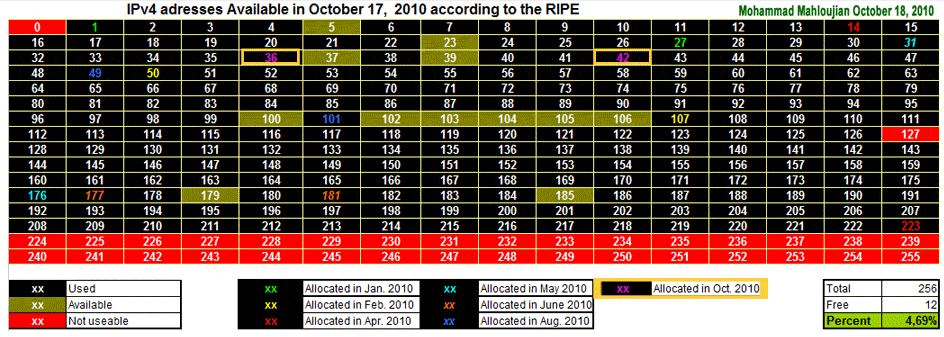
\includegraphics[width=1\linewidth]{./images/ipv4takenaddresses.png}
	\caption{Disponibilità IPv4 del 2010, dal Réseaux IP Européens, ovvero il RIR europeo.}
\end{figure}

\subsection{Funzionalità rimosse}
Nella prossima sezione, andremo a revisionare la struttura dei datagrammi IPv6. Anticipiamo però, quali campi e funzionalità non ritroveremo da IPv4 in quanto rimosse:
\begin{itemize}
	\item \textbf{Frammentazione e riassemblaggio.}\\
	IPv6 \textbf{non consente la frammentazione} e il conseguente \textbf{riassemblaggio nei router intermedi}. Questi passaggi sono \textbf{solo consentiti al mittente e al destinatario}. Quando un router riceve un datagramma IPv6 troppo grande, lo cestina e rimanda al mittente un errore ICMP. Il mittente andrà a frammentare i dati in datagrammi IP più piccoli. La Maximum Transmission Unit minima è 1280 byte, con un consigliato di 1500 byte.
	
	\item \textbf{Checksum dell'header rimosso.}\\
	I protocolli TCP e UDP del livello di trasporto, ed Ethernet, del DLL, implementano già un checksum. Si è quindi preferito \textbf{rimuovere una funzionalità ridondante}.
	
	\item \textbf{TTL - Time To Live.}\\
	Si è deciso di semplificare anche questa funzione, sostituendola con un numero di salti tra router massimo.
	
	\item \textbf{Options.}\\
	Le opzioni aggiuntive per i datagrammi IPv6 sono implementate tramite degli header extra che possono essere aggiunte specificando nel campo "Prossimo header" un numero specifico. Osserveremo dopo questo campo.
\end{itemize}
\newpage

\subsection{Struttura dei datagrammi IPv6}
\begin{figure}[htp]
	\centering
	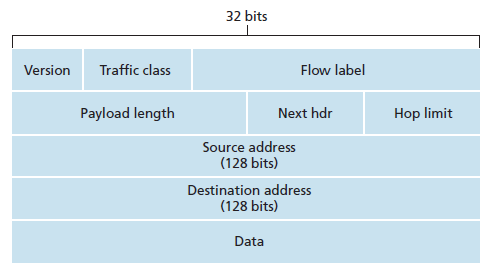
\includegraphics[width=0.75\linewidth]{./images/ipv6structure.png}
\end{figure}

\begin{itemize}
	\item \textbf{Version - Versione.}\\
	Indica la versione di IP usata dal datagramma. 4 bit.
	
	\item \textbf{Traffic Class - Classe di traffico.}\\
	Somiglia al Type of Service di IPv4. Specifica la priorità di un determinato datagramma all'interno di un flusso. VoIP manderà datagrammi di priorità più alta rispetto a SMTP. 8 bit.
	
	\item \textbf{Flow label - Etichetta di flusso.}\\
	Identifica un flusso di datagrammi. 20 bit.
	
	\item \textbf{Payload length - Lunghezza del Payload.}\\
	Interpretato come un unsigned int, indica il numero di byte del datagramma IPv6 a seguire dell'header di dimensione fissa. Il massimo di dati che è possibile trasportare sul payload, è di $2^{16}-1=65,535$. 16 bit. 
	
	\item \textbf{Next header - Prossimo header.}\\
	Specifica il tipo del prossimo header. Questo, può essere l'header del protocollo del livello di trasporto (\verb|TCP: 6, hex 0x06|, \verb|UDP: 17, hex 0x11|), o un header aggiuntivo (\textit{extension header}). Ognuno di questi header aggiuntivi, contiene al suo interno anche il campo \textit{next header}, in modo da poter costruire, su un datagramma, una "catena di header". In questa catena, l'ultimo header aggiuntivo contiene al suo interno il tipo dell'header del livello di trasporto. 8 bit.
	Tra questi header aggiuntivi, abbiamo, ad esempio \verb|Authentication Header (AH): 51| e \\ \verb|Encapsulating Security Payload (ESP): 60|, entrambi meccanismi di \textbf{IPsec}.
	
	\item \textbf{Hop limit - Limite di Hop.}\\
	Un numero che viene decrementato ad ogni inoltro, da parte di router, del datagramma che lo contiene. Quando questo numero diventa 0, viene cestinato. 8 bit.
	
	\item \textbf{Indirizzi.}\\
	Sorgente e destinazione, entrambi a 128 bit.
	
	\item \textbf{Dati.}
\end{itemize}

\newpage

\subsection{Funzionalità di IPv6}
Sintetizziamo in breve gli aspetti \textit{game changer} del protocollo IPv6.
\begin{itemize}
	\item \textbf{Indirizzamento esteso.}\\
	Aumenta la dimensione degli indirizzi. $2^{128}$ indirizzi possibili, praticamente inesauribili. 
	\item \textbf{Unicast, Multicast e Anycast.}\\
	Supporta indizzi unicast, multicast ed anycast. Gli indirizzi multicast e anycast identificano insiemi di interfacce. Mandando un pacchetto a un'indirizzo multicast, questo verrà mandato a tutte le interfacce. Mandando un pacchetto a un'indirizzo anycast, questo verrà all'interfaccia più vicina (o una qualunque).
	\item \textbf{Etichettatura dei flussi.}\\
	Etichettando in un determinato modo i pacchetti di un determinato flusso, diventa possibile dare priorità e offrire delle garanzie di servizio migliori rispetto a determinati protocolli dell'application layer.
	\item \textbf{Rimossa frammentazione ai router intermedi.}
	\item \textbf{Sfoltiti gli header.}
\end{itemize}


\subsection{Sugli indirizzi IPv6}
Per convenzione, i molto più lunghi indirizzi IPv6, rispetto agli IPv4, sono scritti in esadecimale. Otto gruppi da quattro cifre, separati da due punti.

\begin{verbatim}
	esempio di indirizzo IPv6:
	8000:0000:0000:000:0123:4567:89AB:CDEF
	
	o, equivalente:
	8000::123:4567:89AB:CDEF
	
	un indirizzo IPv4 mappato in IPv6:
	::151.97.1.1
	
	indirizzo di loopback:
	::1
	
	non specificato:
	::
\end{verbatim}

\subsubsection{Assegnazione indirizzi IPv6}
\begin{footnotesize}
	\begin{figure}[htp]
		\centering
		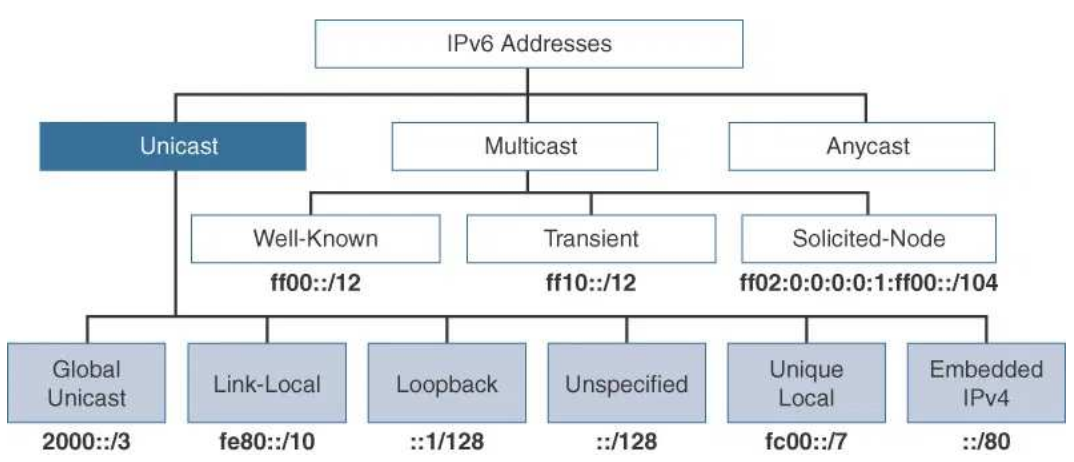
\includegraphics[width=0.85\linewidth]{./images/ipv6indirizzamento.png}
	\end{figure}
\end{footnotesize}
\newpage

\subsection{EUI-64 - Extended Unique Identifier}

L'assegnamento di un indirizzo IPv6 ad un'interfaccia di rete avviene tramite DHPC. Tuttavia, prima dell'assegnamento\footnote{Invece di usare l'indirizzo 0.0.0.0}, questo può essere automaticamente derivato dal suo MAC address a 48 bit, seguendo il metodo \textbf{EUI-64}. \textbf{Utile in configurazioni senza DHCPv6}.

\begin{enumerate}
	\item Si prende l'indirizzo MAC.
	\item Si divide in due metà (24 bit ciascuna).
	\item Si inserisce in mezzo \verb|FF:FE|. (In Windows, vengono inserite delle cifre casuali).
	\item Si cambia il settimo bit (universal/local) del primo byte in 1 se è un indirizzo localmente amministrato, a 0 se è globalmente unico.
\end{enumerate}

Questi indirizzi funzionano solo all'interno di una LAN.
\subsection{Neighbour Discovery Protocol (il nuovo arp!)}
È il protocollo simil-ARP di IPv6. Migliore di ARP, usa ICMPv6, e sfrutta due tipi di messaggi:

\begin{itemize}
	\item \textbf{Neighbour Solicitation (NS).}\\
	Equivalente di un ARP request. Richiede l'indirizzo MAC di un dispositivo con un determinato indirizzo IPv6.
	\item \textbf{Neighbour Advertisement (NA).}\\
	È l'equivalente dell'ARP reply. Può essere anche spontanea senza previa NS, per avvisare i dispositivi di cambiamenti del MAC address.
\end{itemize}
Questo protocollo permette anche di \textbf{autoconfigurare gli host}, e supporta \textbf{Router Advertisement}.

\subsection{IPv6 over Ethernet}
Come IPv4, anche i datagrammi IPv6 viaggiano dentro frame Ethernet. Il pacchetto Ethernet, in questo caso, conterrà nel campo Ethertype il codice \verb|0x86DD|, e non \verb|0x0800| di IPv4.


\subsection{Da IPv4 a IPv6}
L'argomento transizione da IPv4 a IPv6 è un argomento \textbf{delicato}: l'infrastruttura di Internet è stata costruita su IPv4, ma in pochi avrebbero potuto prevedere un tale successo. IPv6 è il sostituto definitivo di IPv4, ma il processo di transizione sarà lento e durerà ancora anni. Non potrà mai essere rapido com'è stato, ad esempio, quello dal protocollo NCP (protocollo di trasporto risalente alla rete ARPANET) a quello TCP.

\subsubsection{Dual Stack}
I dispositivi (host o router) supportano entrambi i protocolli, IPv4 e IPv6. Quello scelto dalle applicazioni dipenderà dal tipo di connessione (con una preferenza verso IPv6).
Questo aumenta la complessità di gestione del nodo, a causa del doppio IP, ma è la soluzione più semplice e stabile.

\subsubsection{Tunneling}
Se i due end-point di una comunicazione supportano IPv6, ma parte della rete che devono attraversare i messaggi no, ciò che si farà, sarà incapsulare l'intero datagramma IPv6 in datagrammi IPv4 prima di essere inoltrato all'interno della rete che supporta IPv4.

\newpage
\section{ICMP - Internet Control Message Protocol}
È un protocollo usato per la trasmissione di informazioni di controllo nella rete. Viene in IP ed è utilizzato per strumenti vari, tra cui \verb!ping! e \verb|traceroute|.
ICMP esiste sia per IPv4 che per IPv6, e in IPv6 trova importante applicazione per i messaggi del \textbf{Neighbor Discovery Protocol}. ICMP include i campi:
\begin{itemize}
	\item \textbf{Tipo.}\\
	Specifica il formato dei messaggi. 8 bit.
	\item \textbf{Codice.}\\
	Identifica il messaggio. 8 bit.
	\item \textbf{Checksum.}\\
	16 bit.
	\item \textbf{Dati.}\\
	La lunghezza di questo campo cambia in base al campo "tipo" e "codice".
\end{itemize}

\section{Firewall}
Sono delle\textbf{ strutture software, hardware o ibride} cui compito è \textbf{bloccare} e/o \textbf{filtrare il traffico malevolo}, in base ai valori relativi ai campi degli header, o effettuano un \textbf{reindirizzamento} per un'ulteriore elaborazione. \textbf{Gestire tutto ciò che costituisce una minaccia per la sicurezza}, e che passa attraverso la rete,\textbf{ è il compito principale dei firewall}, e per adempiere a questo scopo, sono definite delle regole di filtraggio intelligenti, basate su:
\begin{itemize}
	\item Indirizzi IP e porte di origine e destinazione.
	\item Protocolli (TCP, UDP, ICMP...).
	\item Stato della connessione.
	\item \textbf{Contenuto del pacchetto}, in firewall con ispezione profonda.
\end{itemize}

I firewall posso operare a livello di rete, di trasporto e/o al livello applicativo, a seconda delle esigenze di controllo.

\subsection{DMZ - Demilitarized Zone}
Tra una rete locale e una WAN, solitamente, si crea una terza sottorete, chiamata \textbf{Demilitarized Zone}, o \textbf{DMZ}. Questa zona contiene sistemi isolati dalla rete interna, ma raggiungibili dall'esterno, una sorta di \textit{facade} per l'esterno. È qui che i firewall possono:

\begin{itemize}
	\item \textbf{Allow}, far passare un pacchetto.
	\item \textbf{Deny}, bloccare e rispedire un pacchetto al mittente.
	\item \textbf{Drop}, bloccare un pacchetto senza notificarne il mittente. Permette di risparmiare banda. 
\end{itemize}

Un firewall può implementare il NAT, per mascherare gli IP interni alla rete esterna. 
